% ============================================================
% Iskole School Management System — Full Class Diagram
% Compile with: pdflatex class_diagram.tex
% Required packages: tikz, tikz-uml (or pgf-umlcd)
% Install tikz-uml:  place tikz-uml.sty next to this file
%   OR use pgf-umlcd: tlmgr install pgf-umlcd
% ============================================================
\documentclass[a3paper,landscape]{article}
\usepackage[a3paper,landscape,margin=1cm]{geometry}
\usepackage[dvipsnames,svgnames,x11names]{xcolor}
\usepackage{tikz}
\usepackage{pgf-umlcd}   % sudo tlmgr install pgf-umlcd
\usetikzlibrary{positioning, arrows.meta, calc}

% ── Colour palette ──────────────────────────────────────────
\definecolor{CoreBg}      {RGB}{220,234,254}   % light blue  – Core layer
\definecolor{CtrlBg}      {RGB}{220,254,220}   % light green – Controller layer
\definecolor{ModelBg}     {RGB}{254,244,220}   % light amber – Model layer
\definecolor{CoreLine}    {RGB}{ 52,109,219}
\definecolor{CtrlLine}    {RGB}{ 34,139, 34}
\definecolor{ModelLine}   {RGB}{204,120,  0}

\renewcommand{\umlfillcolor}{white}
\renewcommand{\umldrawcolor}{black}

% ── Helper macros ────────────────────────────────────────────
\newcommand{\sep}{\,|\,}

\begin{document}
\pagestyle{empty}

\begin{center}
  {\LARGE\bfseries Iskole School Management System — Class Diagram}\\[4pt]
  {\large Generated: \today}
\end{center}

\vspace{6pt}

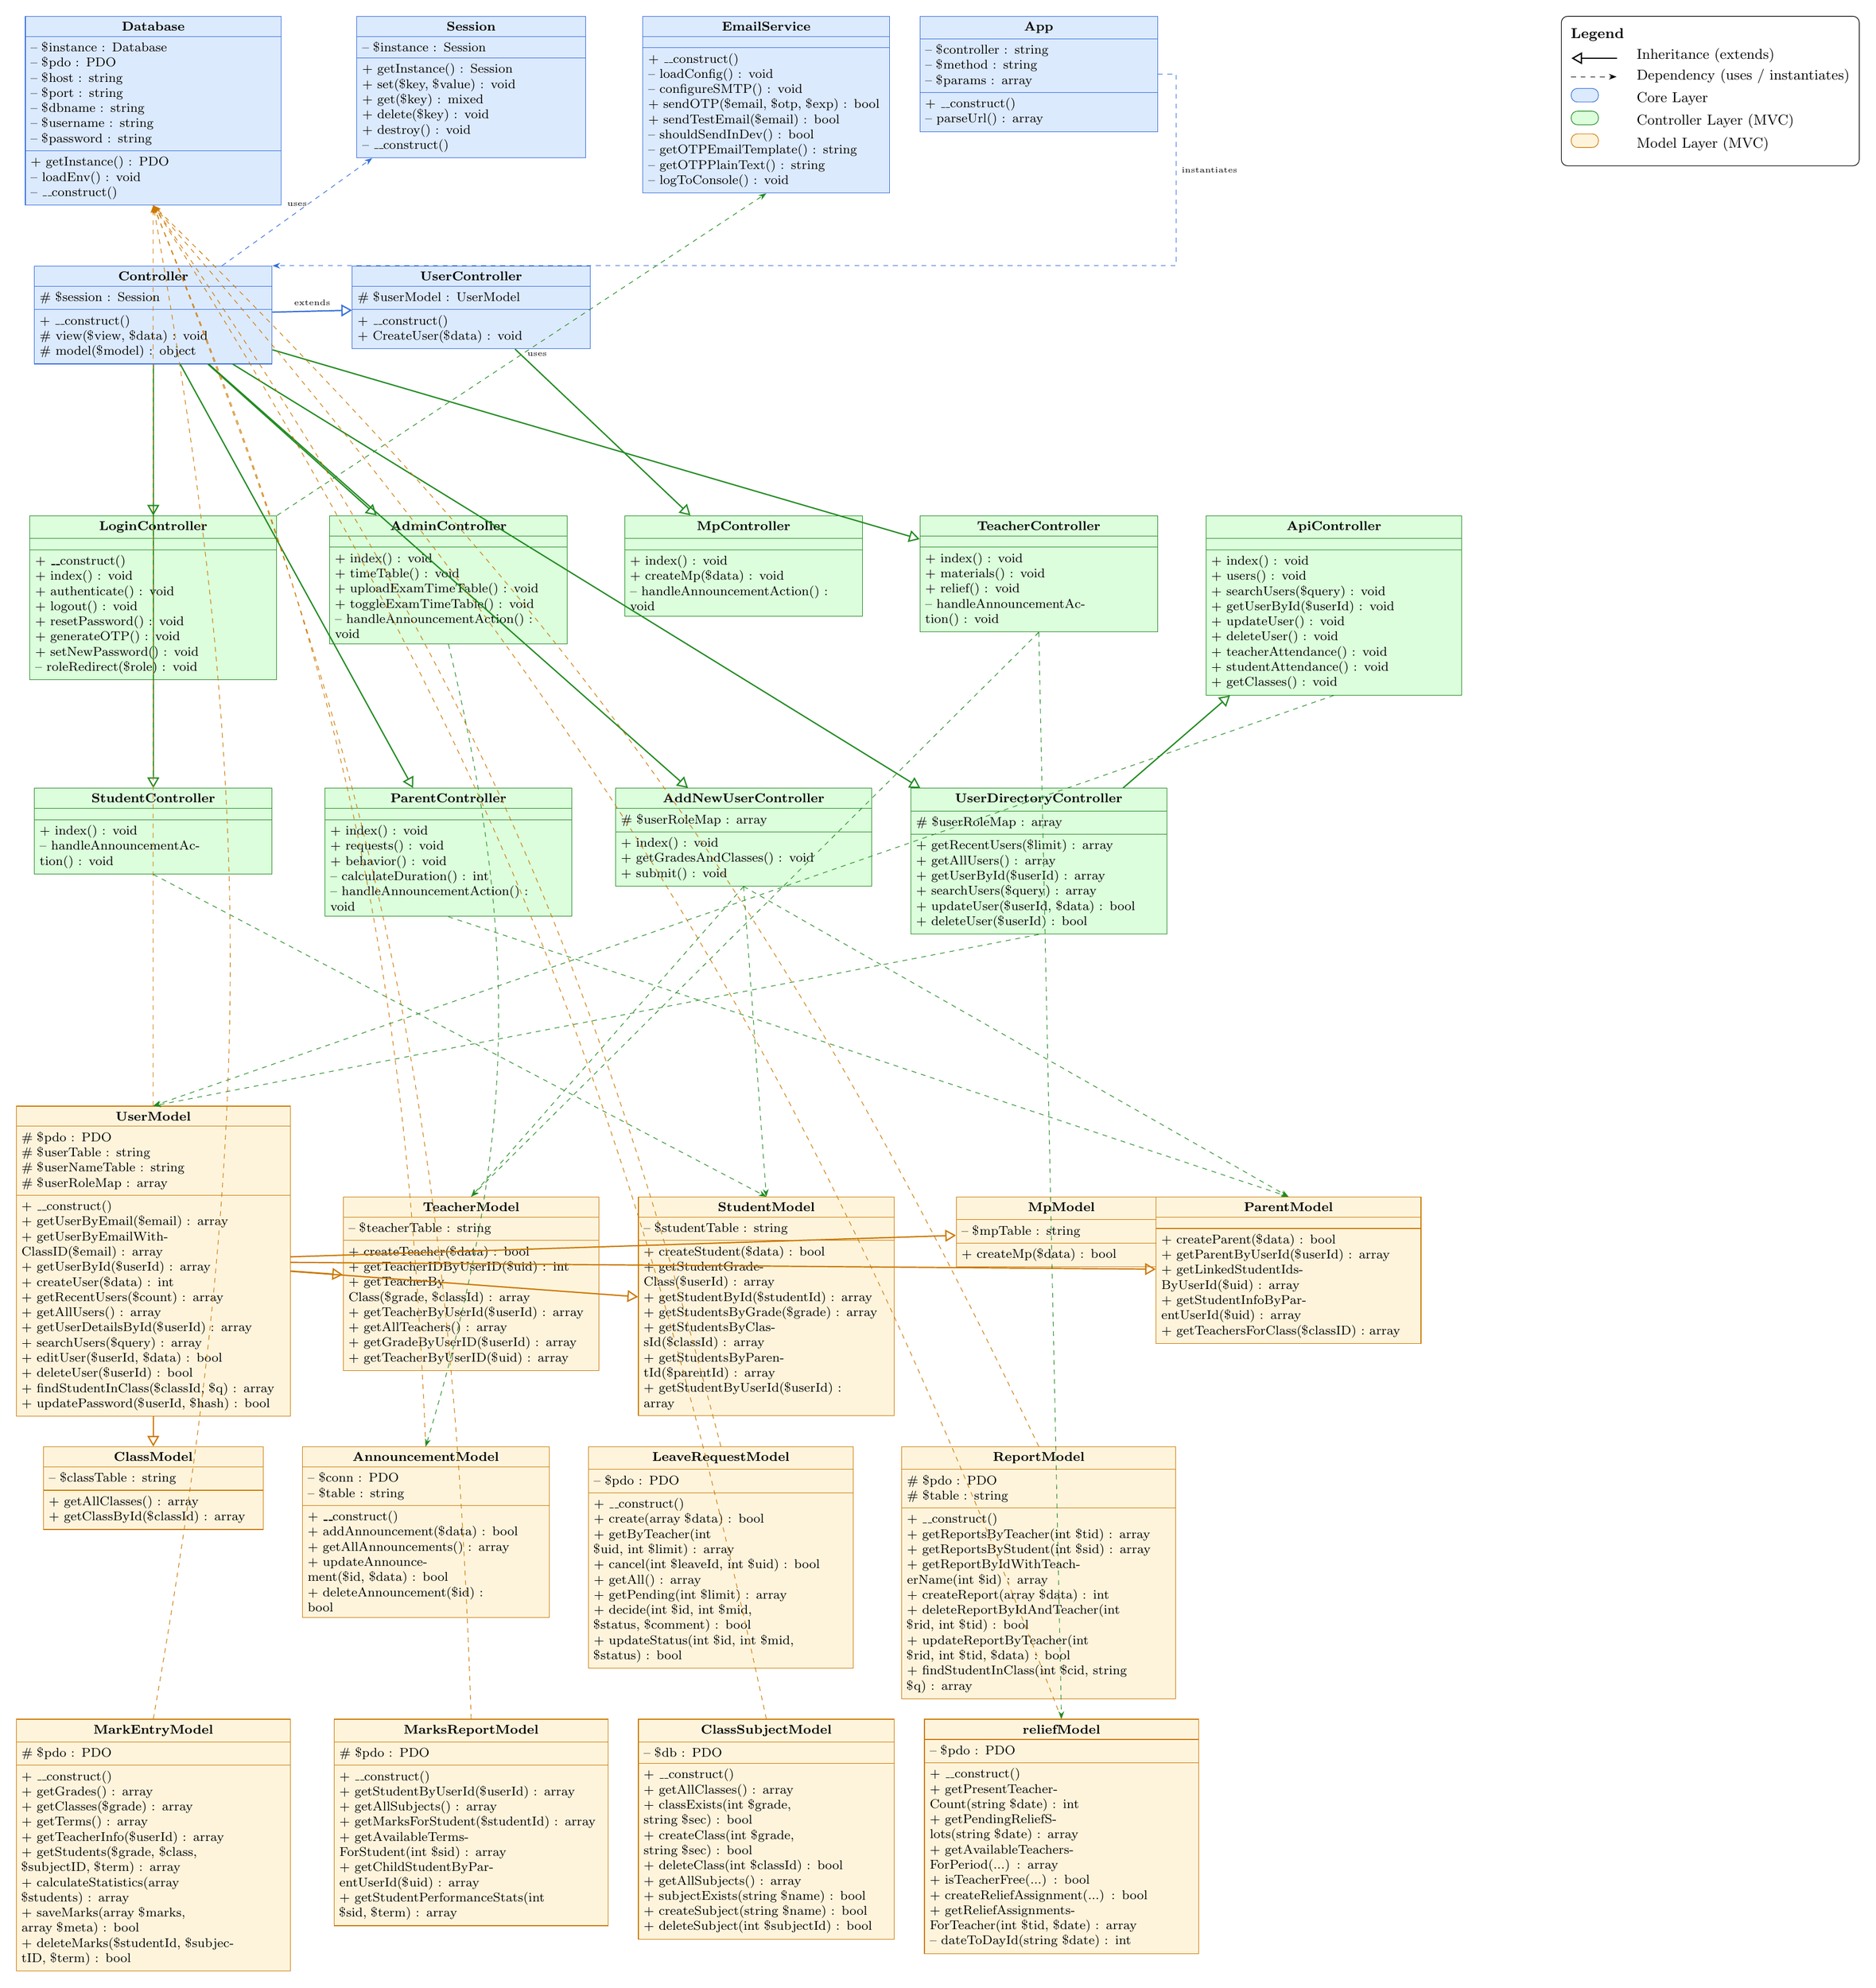
\begin{tikzpicture}[
    font=\footnotesize,
    every node/.style={align=left},
    >=Stealth
  ]

% ════════════════════════════════════════════════════════════
%  CORE LAYER
% ════════════════════════════════════════════════════════════

%% Database (singleton)
\begin{class}[text width=5.4cm, fill=CoreBg, draw=CoreLine]{Database}{0,0}
  \attribute{-- \$instance : Database}
  \attribute{-- \$pdo : PDO}
  \attribute{-- \$host : string}
  \attribute{-- \$port : string}
  \attribute{-- \$dbname : string}
  \attribute{-- \$username : string}
  \attribute{-- \$password : string}
  \operation{+ getInstance() : PDO}
  \operation{-- loadEnv() : void}
  \operation{-- \_\_construct()}
\end{class}

%% Session (singleton)
\begin{class}[text width=4.8cm, fill=CoreBg, draw=CoreLine]{Session}{7,0}
  \attribute{-- \$instance : Session}
  \operation{+ getInstance() : Session}
  \operation{+ set(\$key, \$value) : void}
  \operation{+ get(\$key) : mixed}
  \operation{+ delete(\$key) : void}
  \operation{+ destroy() : void}
  \operation{-- \_\_construct()}
\end{class}

%% EmailService
\begin{class}[text width=5.2cm, fill=CoreBg, draw=CoreLine]{EmailService}{13.5,0}
  \operation{+ \_\_construct()}
  \operation{-- loadConfig() : void}
  \operation{-- configureSMTP() : void}
  \operation{+ sendOTP(\$email, \$otp, \$exp) : bool}
  \operation{+ sendTestEmail(\$email) : bool}
  \operation{-- shouldSendInDev() : bool}
  \operation{-- getOTPEmailTemplate() : string}
  \operation{-- getOTPPlainText() : string}
  \operation{-- logToConsole() : void}
\end{class}

%% App
\begin{class}[text width=5cm, fill=CoreBg, draw=CoreLine]{App}{19.5,0}
  \attribute{-- \$controller : string}
  \attribute{-- \$method : string}
  \attribute{-- \$params : array}
  \operation{+ \_\_construct()}
  \operation{-- parseUrl() : array}
\end{class}

%% Controller (base)
\begin{class}[text width=5cm, fill=CoreBg, draw=CoreLine]{Controller}{0,-5.5}
  \attribute{\# \$session : Session}
  \operation{+ \_\_construct()}
  \operation{\# view(\$view, \$data) : void}
  \operation{\# model(\$model) : object}
\end{class}

%% UserController
\begin{class}[text width=5cm, fill=CoreBg, draw=CoreLine]{UserController}{7,-5.5}
  \attribute{\# \$userModel : UserModel}
  \operation{+ \_\_construct()}
  \operation{+ CreateUser(\$data) : void}
\end{class}

% ── Core relationships ──────────────────────────────────────
\draw[open triangle 60-, thick, draw=CoreLine]
    (UserController) -- (Controller)
    node[midway, above, font=\tiny]{extends};

\draw[->, dashed, draw=CoreLine]
    (Controller) -- (Session)
    node[midway, above, font=\tiny]{uses};

\draw[->, dashed, draw=CoreLine]
    (App.east) -- ++(0.4,0) |- (Controller.north east)
    node[near start, font=\tiny, right]{instantiates};

% ════════════════════════════════════════════════════════════
%  CONTROLLER LAYER
% ════════════════════════════════════════════════════════════

%% LoginController
\begin{class}[text width=5.2cm, fill=CtrlBg, draw=CtrlLine]{LoginController}{0,-11}
  \operation{+ \_\_construct()}
  \operation{+ index() : void}
  \operation{+ authenticate() : void}
  \operation{+ logout() : void}
  \operation{+ resetPassword() : void}
  \operation{+ generateOTP() : void}
  \operation{+ setNewPassword() : void}
  \operation{-- roleRedirect(\$role) : void}
\end{class}

%% AdminController
\begin{class}[text width=5cm, fill=CtrlBg, draw=CtrlLine]{AdminController}{6.5,-11}
  \operation{+ index() : void}
  \operation{+ timeTable() : void}
  \operation{+ uploadExamTimeTable() : void}
  \operation{+ toggleExamTimeTable() : void}
  \operation{-- handleAnnouncementAction() : void}
\end{class}

%% MpController
\begin{class}[text width=5cm, fill=CtrlBg, draw=CtrlLine]{MpController}{13,-11}
  \operation{+ index() : void}
  \operation{+ createMp(\$data) : void}
  \operation{-- handleAnnouncementAction() : void}
\end{class}

%% TeacherController
\begin{class}[text width=5cm, fill=CtrlBg, draw=CtrlLine]{TeacherController}{19.5,-11}
  \operation{+ index() : void}
  \operation{+ materials() : void}
  \operation{+ relief() : void}
  \operation{-- handleAnnouncementAction() : void}
\end{class}

%% StudentController
\begin{class}[text width=5cm, fill=CtrlBg, draw=CtrlLine]{StudentController}{0,-17}
  \operation{+ index() : void}
  \operation{-- handleAnnouncementAction() : void}
\end{class}

%% ParentController
\begin{class}[text width=5.2cm, fill=CtrlBg, draw=CtrlLine]{ParentController}{6.5,-17}
  \operation{+ index() : void}
  \operation{+ requests() : void}
  \operation{+ behavior() : void}
  \operation{-- calculateDuration() : int}
  \operation{-- handleAnnouncementAction() : void}
\end{class}

%% AddNewUserController
\begin{class}[text width=5.4cm, fill=CtrlBg, draw=CtrlLine]{AddNewUserController}{13,-17}
  \attribute{\# \$userRoleMap : array}
  \operation{+ index() : void}
  \operation{+ getGradesAndClasses() : void}
  \operation{+ submit() : void}
\end{class}

%% UserDirectoryController
\begin{class}[text width=5.4cm, fill=CtrlBg, draw=CtrlLine]{UserDirectoryController}{19.5,-17}
  \attribute{\# \$userRoleMap : array}
  \operation{+ getRecentUsers(\$limit) : array}
  \operation{+ getAllUsers() : array}
  \operation{+ getUserById(\$userId) : array}
  \operation{+ searchUsers(\$query) : array}
  \operation{+ updateUser(\$userId, \$data) : bool}
  \operation{+ deleteUser(\$userId) : bool}
\end{class}

%% ApiController
\begin{class}[text width=5.4cm, fill=CtrlBg, draw=CtrlLine]{ApiController}{26,-11}
  \operation{+ index() : void}
  \operation{+ users() : void}
  \operation{+ searchUsers(\$query) : void}
  \operation{+ getUserById(\$userId) : void}
  \operation{+ updateUser() : void}
  \operation{+ deleteUser() : void}
  \operation{+ teacherAttendance() : void}
  \operation{+ studentAttendance() : void}
  \operation{+ getClasses() : void}
\end{class}

% ── Controller inheritance ───────────────────────────────────
\foreach \cls in {LoginController,AdminController,TeacherController,StudentController,ParentController,AddNewUserController,UserDirectoryController}
{
  \draw[open triangle 60-, thick, draw=CtrlLine] (\cls) -- (Controller);
}
\draw[open triangle 60-, thick, draw=CtrlLine] (MpController) -- (UserController);
\draw[open triangle 60-, thick, draw=CtrlLine] (ApiController) -- (UserDirectoryController);

% ── LoginController uses EmailService ───────────────────────
\draw[->, dashed, draw=CtrlLine]
    (LoginController.north east) -- (EmailService.south)
    node[midway, right, font=\tiny]{uses};

% ════════════════════════════════════════════════════════════
%  MODEL LAYER
% ════════════════════════════════════════════════════════════

%% UserModel (base)
\begin{class}[text width=5.8cm, fill=ModelBg, draw=ModelLine]{UserModel}{0,-24}
  \attribute{\# \$pdo : PDO}
  \attribute{\# \$userTable : string}
  \attribute{\# \$userNameTable : string}
  \attribute{\# \$userRoleMap : array}
  \operation{+ \_\_construct()}
  \operation{+ getUserByEmail(\$email) : array}
  \operation{+ getUserByEmailWithClassID(\$email) : array}
  \operation{+ getUserById(\$userId) : array}
  \operation{+ createUser(\$data) : int}
  \operation{+ getRecentUsers(\$count) : array}
  \operation{+ getAllUsers() : array}
  \operation{+ getUserDetailsById(\$userId) : array}
  \operation{+ searchUsers(\$query) : array}
  \operation{+ editUser(\$userId, \$data) : bool}
  \operation{+ deleteUser(\$userId) : bool}
  \operation{+ findStudentInClass(\$classId, \$q) : array}
  \operation{+ updatePassword(\$userId, \$hash) : bool}
\end{class}

%% TeacherModel
\begin{class}[text width=5.4cm, fill=ModelBg, draw=ModelLine]{TeacherModel}{7,-26}
  \attribute{-- \$teacherTable : string}
  \operation{+ createTeacher(\$data) : bool}
  \operation{+ getTeacherIDByUserID(\$uid) : int}
  \operation{+ getTeacherByClass(\$grade, \$classId) : array}
  \operation{+ getTeacherByUserId(\$userId) : array}
  \operation{+ getAllTeachers() : array}
  \operation{+ getGradeByUserID(\$userId) : array}
  \operation{+ getTeacherByUserID(\$uid) : array}
\end{class}

%% StudentModel
\begin{class}[text width=5.4cm, fill=ModelBg, draw=ModelLine]{StudentModel}{13.5,-26}
  \attribute{-- \$studentTable : string}
  \operation{+ createStudent(\$data) : bool}
  \operation{+ getStudentGradeClass(\$userId) : array}
  \operation{+ getStudentById(\$studentId) : array}
  \operation{+ getStudentsByGrade(\$grade) : array}
  \operation{+ getStudentsByClassId(\$classId) : array}
  \operation{+ getStudentsByParentId(\$parentId) : array}
  \operation{+ getStudentByUserId(\$userId) : array}
\end{class}

%% MpModel
\begin{class}[text width=4.4cm, fill=ModelBg, draw=ModelLine]{MpModel}{20,-26}
  \attribute{-- \$mpTable : string}
  \operation{+ createMp(\$data) : bool}
\end{class}

%% ParentModel
\begin{class}[text width=5.6cm, fill=ModelBg, draw=ModelLine]{ParentModel}{25,-26}
  \operation{+ createParent(\$data) : bool}
  \operation{+ getParentByUserId(\$userId) : array}
  \operation{+ getLinkedStudentIdsByUserId(\$uid) : array}
  \operation{+ getStudentInfoByParentUserId(\$uid) : array}
  \operation{+ getTeachersForClass(\$classID) : array}
\end{class}

%% ClassModel
\begin{class}[text width=4.6cm, fill=ModelBg, draw=ModelLine]{ClassModel}{0,-31.5}
  \attribute{-- \$classTable : string}
  \operation{+ getAllClasses() : array}
  \operation{+ getClassById(\$classId) : array}
\end{class}

%% AnnouncementModel
\begin{class}[text width=5.2cm, fill=ModelBg, draw=ModelLine]{AnnouncementModel}{6,-31.5}
  \attribute{-- \$conn : PDO}
  \attribute{-- \$table : string}
  \operation{+ \_\_construct()}
  \operation{+ addAnnouncement(\$data) : bool}
  \operation{+ getAllAnnouncements() : array}
  \operation{+ updateAnnouncement(\$id, \$data) : bool}
  \operation{+ deleteAnnouncement(\$id) : bool}
\end{class}

%% LeaveRequestModel
\begin{class}[text width=5.6cm, fill=ModelBg, draw=ModelLine]{LeaveRequestModel}{12.5,-31.5}
  \attribute{-- \$pdo : PDO}
  \operation{+ \_\_construct()}
  \operation{+ create(array \$data) : bool}
  \operation{+ getByTeacher(int \$uid, int \$limit) : array}
  \operation{+ cancel(int \$leaveId, int \$uid) : bool}
  \operation{+ getAll() : array}
  \operation{+ getPending(int \$limit) : array}
  \operation{+ decide(int \$id, int \$mid, \$status, \$comment) : bool}
  \operation{+ updateStatus(int \$id, int \$mid, \$status) : bool}
\end{class}

%% ReportModel
\begin{class}[text width=5.8cm, fill=ModelBg, draw=ModelLine]{ReportModel}{19.5,-31.5}
  \attribute{\# \$pdo : PDO}
  \attribute{\# \$table : string}
  \operation{+ \_\_construct()}
  \operation{+ getReportsByTeacher(int \$tid) : array}
  \operation{+ getReportsByStudent(int \$sid) : array}
  \operation{+ getReportByIdWithTeacherName(int \$id) : array}
  \operation{+ createReport(array \$data) : int}
  \operation{+ deleteReportByIdAndTeacher(int \$rid, int \$tid) : bool}
  \operation{+ updateReportByTeacher(int \$rid, int \$tid, \$data) : bool}
  \operation{+ findStudentInClass(int \$cid, string \$q) : array}
\end{class}

%% MarkEntryModel
\begin{class}[text width=5.8cm, fill=ModelBg, draw=ModelLine]{MarkEntryModel}{0,-37.5}
  \attribute{\# \$pdo : PDO}
  \operation{+ \_\_construct()}
  \operation{+ getGrades() : array}
  \operation{+ getClasses(\$grade) : array}
  \operation{+ getTerms() : array}
  \operation{+ getTeacherInfo(\$userId) : array}
  \operation{+ getStudents(\$grade, \$class, \$subjectID, \$term) : array}
  \operation{+ calculateStatistics(array \$students) : array}
  \operation{+ saveMarks(array \$marks, array \$meta) : bool}
  \operation{+ deleteMarks(\$studentId, \$subjectID, \$term) : bool}
\end{class}

%% MarksReportModel
\begin{class}[text width=5.8cm, fill=ModelBg, draw=ModelLine]{MarksReportModel}{7,-37.5}
  \attribute{\# \$pdo : PDO}
  \operation{+ \_\_construct()}
  \operation{+ getStudentByUserId(\$userId) : array}
  \operation{+ getAllSubjects() : array}
  \operation{+ getMarksForStudent(\$studentId) : array}
  \operation{+ getAvailableTermsForStudent(int \$sid) : array}
  \operation{+ getChildStudentByParentUserId(\$uid) : array}
  \operation{+ getStudentPerformanceStats(int \$sid, \$term) : array}
\end{class}

%% ClassSubjectModel
\begin{class}[text width=5.4cm, fill=ModelBg, draw=ModelLine]{ClassSubjectModel}{13.5,-37.5}
  \attribute{-- \$db : PDO}
  \operation{+ \_\_construct()}
  \operation{+ getAllClasses() : array}
  \operation{+ classExists(int \$grade, string \$sec) : bool}
  \operation{+ createClass(int \$grade, string \$sec) : bool}
  \operation{+ deleteClass(int \$classId) : bool}
  \operation{+ getAllSubjects() : array}
  \operation{+ subjectExists(string \$name) : bool}
  \operation{+ createSubject(string \$name) : bool}
  \operation{+ deleteSubject(int \$subjectId) : bool}
\end{class}

%% reliefModel
\begin{class}[text width=5.8cm, fill=ModelBg, draw=ModelLine]{reliefModel}{20,-37.5}
  \attribute{-- \$pdo : PDO}
  \operation{+ \_\_construct()}
  \operation{+ getPresentTeacherCount(string \$date) : int}
  \operation{+ getPendingReliefSlots(string \$date) : array}
  \operation{+ getAvailableTeachersForPeriod(...) : array}
  \operation{+ isTeacherFree(...) : bool}
  \operation{+ createReliefAssignment(...) : bool}
  \operation{+ getReliefAssignmentsForTeacher(int \$tid, \$date) : array}
  \operation{-- dateToDayId(string \$date) : int}
\end{class}

% ── Model inheritance ────────────────────────────────────────
\foreach \cls in {TeacherModel,StudentModel,MpModel,ParentModel,ClassModel}
{
  \draw[open triangle 60-, thick, draw=ModelLine] (\cls) -- (UserModel);
}

% ── Models depend on Database ────────────────────────────────
\foreach \cls in {AnnouncementModel,LeaveRequestModel,ReportModel,MarkEntryModel,MarksReportModel,ClassSubjectModel,reliefModel}
{
  \draw[->, dashed, draw=ModelLine, bend right=10]
      (\cls.north) to (Database.south);
}
\draw[->, dashed, draw=ModelLine]
    (UserModel.north) -- ++(0,0.4) -| (Database.south);

% ── Controller→Model usage arrows (selected key ones) ─────────
\draw[->, dashed, draw=CtrlLine, bend left=15]
    (AdminController.south) to (AnnouncementModel.north);
\draw[->, dashed, draw=CtrlLine]
    (TeacherController.south) to (TeacherModel.north);
\draw[->, dashed, draw=CtrlLine]
    (TeacherController.south) to (reliefModel.north);
\draw[->, dashed, draw=CtrlLine]
    (StudentController.south) to (StudentModel.north);
\draw[->, dashed, draw=CtrlLine]
    (ParentController.south) to (ParentModel.north);
\draw[->, dashed, draw=CtrlLine]
    (ApiController.south) to (UserModel.north);
\draw[->, dashed, draw=CtrlLine]
    (AddNewUserController.south) to (TeacherModel.north);
\draw[->, dashed, draw=CtrlLine]
    (AddNewUserController.south) to (StudentModel.north);
\draw[->, dashed, draw=CtrlLine]
    (AddNewUserController.south) to (ParentModel.north);
\draw[->, dashed, draw=CtrlLine]
    (UserDirectoryController.south) to (UserModel.north);

% ════════════════════════════════════════════════════════════
%  LEGEND
% ════════════════════════════════════════════════════════════
\node[draw, fill=white, rounded corners, inner sep=6pt,
      font=\small,
      anchor=north west] at (31, 0) {%
  \begin{tabular}{@{}ll@{}}
    \multicolumn{2}{@{}l@{}}{\textbf{Legend}} \\[2pt]
    \tikz\draw[open triangle 60-, thick] (0,0) -- (1,0); & Inheritance (extends) \\[2pt]
    \tikz\draw[->, dashed]               (0,0) -- (1,0); & Dependency (uses / instantiates) \\[2pt]
    \tikz\fill[CoreBg, draw=CoreLine]    (0,0) rectangle (0.6,0.3); & Core Layer \\[2pt]
    \tikz\fill[CtrlBg, draw=CtrlLine]    (0,0) rectangle (0.6,0.3); & Controller Layer (MVC) \\[2pt]
    \tikz\fill[ModelBg, draw=ModelLine]  (0,0) rectangle (0.6,0.3); & Model Layer (MVC) \\[2pt]
  \end{tabular}%
};

\end{tikzpicture}

\end{document}
